\documentclass[a4paper,twoside]{report}
\usepackage[utf8]{inputenc}  
\usepackage[T1]{fontenc}
\usepackage{graphicx}
\usepackage{tikz}
\usepackage[top=2cm, bottom=2cm, left=2cm, right=2cm]{geometry}
\usepackage{hyperref}
\usepackage{multicol}
\usepackage{multirow}
\usepackage{caption}
\usepackage{rotating}
\usepackage{colortbl}



\setlength{\parindent}{0.5cm}
\begin{document}
\title{Projet d'imagerie multispectrale par satelitte}
\author{Le Vaou Youna, David Pierre, Barbotin Aurélien, Michelland Benjamin}
\date\today
\maketitle
\chapter{État de l'art}
\section{Machine Learning}
\textit{L'apprentissage automatique (machine learning en anglais), champ d'étude de l'intelligence artificielle, concerne la conception, l'analyse, le développement et l'implémentation de méthodes permettant à une machine (au sens large) d'évoluer par un processus systématique, et ainsi de remplir des tâches difficiles ou impossibles à remplir par des moyens algorithmiques plus classiques.\footnote{\href{https://fr.wikipedia.org/wiki/Apprentissage_automatique}{Apprentissage automatique}}}
\subsection{Les algorithmes}
\paragraph{Les principes globaux\\}
Il existe plusieurs familles d'algorithmes qui peuvent être utilisés pour l'apprentissage supervisé, on différenciera dans un premier temps les algorithmes linéaires et non-linéaires. Dans la famille des algorithmes non-linéaire, on trouve des algorithmes intrinsèquement multi-classes (tel que l'algorithme dis des k-plus proches voisins que nous détaillerons plus tard), et les algorithmes binaires.\newline
\label{DiagAlg}
\begin{center}
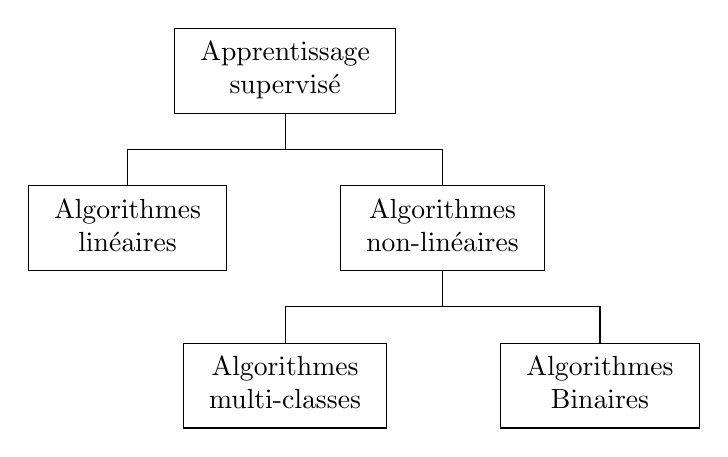
\begin{tikzpicture}
\begin{scope}
\node (AS) at (0,4.9) [rectangle,draw] {\begin{tabular}{c}Apprentissage\\ supervisé\end{tabular} };
\node (ASL) at (-2,2.9) [rectangle,draw] {\begin{tabular}{c}Algorithmes\\ linéaires\end{tabular} };
\node (ASNL) at (2,2.9) [rectangle,draw] {\begin{tabular}{c}Algorithmes\\ non-linéaires\end{tabular} };
\node (ASIM) at (0,0.9) [rectangle,draw] {\begin{tabular}{c}Algorithmes\\ multi-classes\end{tabular} };
\node (ASNM) at (4,0.9) [rectangle,draw] {\begin{tabular}{c}Algorithmes\\Binaires\end{tabular} };
\draw (AS) -- (0,3.9);
\draw (0,3.9) -| (ASNL);
\draw (0,3.9) -| (ASL);
\draw (ASNL) -- (2,1.9);
\draw (2,1.9) -| (ASIM);
\draw (2,1.9) -| (ASNM);
\end{scope}
\end{tikzpicture}
\captionof{figure}{Diagramme des différents algorithme de classification.}
\end{center}

\paragraph{}
Les algorithmes intrinsèquement multi-classes se suffisent à eux même, dans le sens où il suffit d'appliquer l'algorithme à l'ensemble des échantillons d'entraînement pour obtenir une classification complète.\newpage
\paragraph{}
Les algorithmes binaires, quand à eux demande un peu plus de travail, dès que l'on veut traiter plus de deux classe, il faut faire plusieurs entraînements, en se ramenant chaque fois à un problème binaire. La encore, il y deux approche possible en fonction en fonction des algorithmes :
 \begin{itemize}
   \item[>] La première approche est appelé un contre tous, elle consiste comme son nom l'indique, à prendre chaque classe et à l'opposer à l'ensemble des autres classe. On obtient alors n problèmes binaires et pour un élément à classifier, en cas d'ambiguïté, la classe qui obtient le plus de "vote" favorable est choisie;
   \item[>] La seconde méthode est celle du un contre un, toutes les classes sont "opposée" successivement, deux à deux, et de la même façon c'est la classe qui obtient le plus de "vote" favorable qui est choisie. La principale différence réside dans le fait qu'il y a dans ce cas ${n \choose 2}=\frac{n(n-1)}{2}$ entraînement à réaliser.
 \end{itemize}
\paragraph{Les classifications linéaires\\}
Réaliser une classification linéaire d'un ensemble de données en différentes classes revient en deux dimensions à trouver la droite qui sépare au mieux deux ensembles de vecteurs.\newline
\begin{center}
 \begin{tikzpicture}
 \begin{scope}
 \draw[latex-latex, thin, draw=gray] (-4,0)--(4,0) node [right] {$x$}; % l'axe des abscisses
 \draw[latex-latex, thin, draw=gray] (0,-4)--(0,4) node [above] {$y$}; % l'axe des ordonnées
 \draw[thick] (-4,-4)--(4,4); % la courbe

\foreach \Point in {(-2,2), (-2,1.8), (-2,2.2), (-1.5,2), (-1.8,2.2),(-1.5,2.2),(-1.8,2),(-2.2,2),(-2,1.5),(-1.8,1.8)}{
    \node [blue] at \Point {\textbullet};
}

\foreach \Point in {(2,-2), (2,-1.8), (2,-2.2), (1.5,-2), (1.8,-2.2),(1.5,-2.2),(1.8,-2),(2.2,-2),(2,-1.5),(1.8,-1.8)}{
    \node [red] at \Point {\textbullet};
}

% to ensure that the points are being properly centered:
\draw [dotted, gray] (-4,-4) grid (4,4);
 \end{scope}
\end{tikzpicture}
\end{center}
il existe plusieurs méthodes pour trouver une droite qui sépare correctement les deux ensembles de points :
\begin{itemize}
  \item[>] La première méthode consiste à faire l'hypothèse que tous les point des deux ensembles sont alignés, et qu'on peut alors trouver une droite telle que tous les points soit à une distance de 1, pour une des deux classes, et de -1 pour l'autre. On se ramène alors à une optimisation linéaire qui peut-être résolue par exemple par la méthode des moindres carrés.
  \item[>] Une seconde méthode consiste à utiliser l'analyse discriminante linéaire\footnote{ou analyse discriminante de Fisher}(LDA), cette analyse consiste à poser l'hypothèse que chaque ensemble de points à une distribution gaussienne, et à trouver, à partir de la variance et de la moyenne de ces distribution la meilleur séparation entre les ensembles. Cependant, l'hypothèse de distribution gaussienne nous pousse à considérer uniquement un apprentissage de type un contre un et donc a faire plus d'entraînement.
\end{itemize}
\paragraph{Les classification non-linéaires\newline}
Support Vecteur Machine (SVM) : 
Random forest :
k-nearest neighbors :
\subsection{L'évaluation}
Une classification peut-être appliquée à n'importe quel ensemble de données, il y trois critère d'évaluation d'un classification, sa précision, sa répétabilité et sa généralisation. Pour 
\end{document}
